\section{\ac{SAT}-solvers}

\renewcommand{\CURPATH}{basics/SAT}

SMT vs. SAT is like high level \ac{PL} vs. assembly language.
The latter can be much more efficient, but it's hard to program in it.

SAT is abbreviation of ``Boolean satisfiability problem''.
The problem is to find such a set of variables, which, if plugged into boolean expression, will result in ``true''.

\subsection{CNF form}

\ac{CNF}\footnote{\url{https://en.wikipedia.org/wiki/Conjunctive_normal_form}} is a \emph{normal form}.

% TODO recheck
% TODO write abt it!
%\emph{normal form} is somewhat similar to polynomials in algebra. 
%What is polynomial?
%It is a standard way to express unsystematic equations like $2x \cdot x$ as $3x$ polynomial, 
%and so you will be able to apply some operations to polynomials like summing, etc.

Any boolean expression can be converted to \emph{normal form} and \ac{CNF} is one of them.
The \ac{CNF} expression is a bunch of clauses (sub-expressions) constisting of terms (variables), ORs and NOTs, 
all of which are then glued together with AND into a full expression.
There is a way to memorize it: \ac{CNF} is ``AND of ORs'' (or ``product of sums'') and \ac{DNF} is ``OR of ANDs'' (or ``sum of products'').

Example is: $(\neg A \vee B) \wedge (C \vee \neg D)$.

$\vee$ stands for OR (logical disjunction\footnote{\url{https://en.wikipedia.org/wiki/Logical_disjunction}}), 
``+'' sign is also sometimes used for OR.

$\wedge$ stands for AND (logical conjunction\footnote{\url{https://en.wikipedia.org/wiki/Logical_conjunction}}).
It is easy to memorize: $\wedge$ looks like ``A'' letter.
``$\cdot$'' is also sometimes used for AND.

$\neg$ is negation (NOT).

% TODO A/B is the first clause, C/D is second

\subsection{Example: 2-bit adder}
\label{adder}

\ac{SAT}-solver is merely a solver of huge boolean equations in CNF form.
It just gives the answer, if there is a set of input values which can satisfy CNF expression, and what input values must be.

Here is a 2-bit adder for example:

\begin{figure}[ht!]
\centering
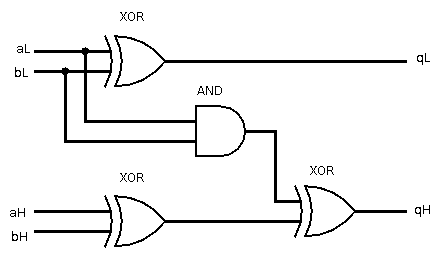
\includegraphics[scale=0.75]{\CURPATH/adder_logisim.png}
\caption{2-bit adder circuit}
\end{figure}

The adder in its simplest form: it has no carry-in and carry-out, and it has 3 XOR gates and one AND gate.
Let's try to figure out, which sets of input values will force adder to set both two output bits?
By doing quick memory calculation, we can see that there are 4 ways to do so: $0+3=3$, $1+2=3$, $2+1=3$, $3+0=3$.
Here is also truth table, with these rows highlighted:

\newcommand{\HLcell}{\cellcolor{blue!25}}

\begin{center}
\begin{doublespace}
\noindent\(\begin{array}{l|llllll}
  & \text{aH} & \text{aL} & \text{bH} & \text{bL} & \text{qH} & \text{qL} \\
\hline
 \text{3+3 = 6 $\equiv $ 2 (mod 4)} & 1 & 1 & 1 & 1 & 1 & 0 \\
 \text{3+2 = 5 $\equiv $ 1 (mod 4)} & 1 & 1 & 1 & 0 & 0 & 1 \\
 \text{3+1 = 4 $\equiv $ 0 (mod 4)} & 1 & 1 & 0 & 1 & 0 & 0 \\
 \text{\HLcell{}3+0 = 3 $\equiv $ 3 (mod 4)} & \HLcell{}1 & \HLcell{}1 & \HLcell{}0 & \HLcell{}0 & \HLcell{}1 & \HLcell{}1 \\
 \text{2+3 = 5 $\equiv $ 1 (mod 4)} & 1 & 0 & 1 & 1 & 0 & 1 \\
 \text{2+2 = 4 $\equiv $ 0 (mod 4)} & 1 & 0 & 1 & 0 & 0 & 0 \\
 \text{\HLcell{}2+1 = 3 $\equiv $ 3 (mod 4)} & \HLcell{}1 & \HLcell{}0 & \HLcell{}0 & \HLcell{}1 & \HLcell{}1 & \HLcell{}1 \\
 \text{2+0 = 2 $\equiv $ 2 (mod 4)} & 1 & 0 & 0 & 0 & 1 & 0 \\
 \text{1+3 = 4 $\equiv $ 0 (mod 4)} & 0 & 1 & 1 & 1 & 0 & 0 \\
 \text{\HLcell{}1+2 = 3 $\equiv $ 3 (mod 4)} & \HLcell{}0 & \HLcell{}1 & \HLcell{}1 & \HLcell{}0 & \HLcell{}1 & \HLcell{}1 \\
 \text{1+1 = 2 $\equiv $ 2 (mod 4)} & 0 & 1 & 0 & 1 & 1 & 0 \\
 \text{1+0 = 1 $\equiv $ 1 (mod 4)} & 0 & 1 & 0 & 0 & 0 & 1 \\
 \text{\HLcell{}0+3 = 3 $\equiv $ 3 (mod 4)} & \HLcell{}0 & \HLcell{}0 & \HLcell{}1 & \HLcell{}1 & \HLcell{}1 & \HLcell{}1 \\
 \text{0+2 = 2 $\equiv $ 2 (mod 4)} & 0 & 0 & 1 & 0 & 1 & 0 \\
 \text{0+1 = 1 $\equiv $ 1 (mod 4)} & 0 & 0 & 0 & 1 & 0 & 1 \\
 \text{0+0 = 0 $\equiv $ 0 (mod 4)} & 0 & 0 & 0 & 0 & 0 & 0 \\
\end{array}\)
\end{doublespace}
\end{center}


Let's find, what \ac{SAT}-solver can say about it?

First, we should represent our 2-bit adder as \ac{CNF} expression.

Using Wolfram Mathematica, we can express 1-bit expression for both adder outputs:\\
\\
\textbf{\texttt{In[]:=AdderQ0[aL$\_$,bL$\_$]=Xor[aL,bL]}} \\
\textbf{\texttt{Out[]:=aL $\veebar$ bL}} \\
\\
\textbf{\texttt{In[]:=AdderQ1[aL$\_$,aH$\_$,bL$\_$,bH$\_$]=Xor[And[aL,bL],Xor[aH,bH]]}} \\
\textbf{\texttt{Out[]:=aH $\veebar$ bH $\veebar$ (aL \&\& bL)}} \\
\\
We need such expression, where both parts will generate 1's.
Let's use Wolfram Mathematica find all instances of such expression (I glueled both parts with And): \\
\\
\textbf{\texttt{In[]:=Boole[SatisfiabilityInstances[And[AdderQ0[aL,bL],AdderQ1[aL,aH,bL,bH]],\{aL,aH,bL,bH\},4]]}} \\
\textbf{\texttt{Out[]:=\{1,1,0,0\},\{1,0,0,1\},\{0,1,1,0\},\{0,0,1,1\}}} \\
\\
Yes, indeed, Mathematica says, there are 4 inputs which will lead to the result we need.
So, Mathematica can also be used as \ac{SAT} solver.

Nevertheless, let's proceed to \ac{CNF} form. Using Mathematica again, let's convert our expression to \ac{CNF} form:\\
\\
\textbf{\texttt{In[]:=cnf=BooleanConvert[And[AdderQ0[aL,bL],AdderQ1[aL,aH,bL,bH]],``CNF'']}} \\
\textbf{\texttt{Out[]:=(!aH $\|$ !bH) \&\& (aH $\|$ bH) \&\& (!aL $\|$ !bL) \&\& (aL $\|$ bL)}} \\
\\
Looks more complex. The reason of such verbosity is that \ac{CNF} form doesn't allow XOR operations.
% FIXME: TeX form of the expression!

\subsubsection{MiniSat}

For starters, we can try MiniSat\footnote{\url{http://minisat.se/MiniSat.html}}.
The standard way to encode \ac{CNF} expression for MiniSat is to enumerate all OR parts at each line.
Also, MiniSat doesn't support variable names, just numbers.
Let's enumerate our variables: 1 will be aH, 2 -- aL, 3 -- bH, 4 -- bL.

Here is what I've got when I converted Mathematica expression to the MiniSat input file:

\lstinputlisting{\CURPATH/adder.cnf}

Two 4's at the first lines are number of variables and number of clauses respectively.
There are 4 lines then, each for each OR clause.
Minus before variable number meaning that the variable is negated.
Absence of minus -- not negated.
Zero at the end is just terminating zero, meaning end of the clause.

In other words, each line is OR-clause with optional negations,
and the task of MiniSat is to find such set of input, which can satisfy all lines in the input file.

That file I named as \emph{adder.cnf} and now let's try MiniSat:

\begin{lstlisting}
% minisat -verb=0 adder.cnf results.txt
SATISFIABLE
\end{lstlisting}

The results are in \emph{results.txt} file:

\begin{lstlisting}
SAT
-1 -2 3 4 0
\end{lstlisting}

This means, if the first two variables (aH and aL) will be \emph{false}, and the last two variables (bH and bL) will be set to \emph{true},
the whole \ac{CNF} expression is satisfiable.
Seems to be true: if bH and bL are the only inputs set to \emph{true}, both resulting bits are also has \emph{true} states.

Now how to get other instances? \ac{SAT}-solvers, like \ac{SMT} solvers, produce only one solution (or \emph{instance}).

MiniSat uses \ac{PRNG} and its initial seed can be set explicitely. I tried different values, but result is still the same.
Nevertheless, CryptoMiniSat in this case was able to show all possible 4 instances, in chaotic order, though.
So this is not very robust way.

Perhaps, the only known way is to negate solution clause and add it to the input expression.
We've got \TT{-1 -2 3 4}, 
now we can negate all values in it (just toggle minuses: \TT{1 2 -3 -4}) and add it to the end of the input file:

\begin{lstlisting}
p cnf 4 5
-1 -3 0
1 3 0
-2 -4 0
2 4 0
1 2 -3 -4
\end{lstlisting}

Now we've got another result:

\begin{lstlisting}
SAT
1 2 -3 -4 0
\end{lstlisting}

This means, aH and aL must be both \emph{true} and bH and bL must be \emph{false}, to satisfy the input expression.
Let's negate this clause and add it again:

\begin{lstlisting}
p cnf 4 6
-1 -3 0
1 3 0
-2 -4 0
2 4 0
1 2 -3 -4
-1 -2 3 4 0
\end{lstlisting}

The result is:

\begin{lstlisting}
SAT
-1 2 3 -4 0
\end{lstlisting}

aH=false, aL=true, bH=true, bL=false. This is also correct, according to our truth table.

Let's add it again:

\begin{lstlisting}
p cnf 4 7
-1 -3 0
1 3 0
-2 -4 0
2 4 0
1 2 -3 -4
-1 -2 3 4 0
1 -2 -3 4 0
\end{lstlisting}

\begin{lstlisting}
SAT
1 -2 -3 4 0
\end{lstlisting}

\emph{aH=true, aL=false, bH=false, bL=true.} This is also correct.

This is fourth result. There are shouldn't be more. What if to add it?

\begin{lstlisting}
p cnf 4 8
-1 -3 0
1 3 0
-2 -4 0
2 4 0
1 2 -3 -4
-1 -2 3 4 0
1 -2 -3 4 0
-1 2 3 -4 0
\end{lstlisting}

Now MiniSat just says ``UNSATISFIABLE'' without any additional information in the resulting file.

Our example is tiny, but MiniSat can work with huge \ac{CNF} expressions.

\subsubsection{CryptoMiniSat}

XOR operation is absent in \ac{CNF} form, but crucial in cryptographical algorithms.
Simplest possible way to represent single XOR operation in \ac{CNF} form is:
$(\neg x \vee \neg y) \wedge (x \vee y)$ -- not that small expression, 
though, many XOR operations in single expression can be optimized better.

One significant difference between MiniSat and CryptoMiniSat is that
the latter supports clauses with XOR operations instead of ORs,
because CryptoMiniSat has aim to analyze crypto algorithms\footnote{\url{http://www.msoos.org/xor-clauses/}}.
XOR clauses are handled by CryptoMiniSat in a special way without translating to OR clauses.

You need just to prepend a clause with ``x'' in \ac{CNF} file and OR clause is then treated as XOR clause by CryptoMiniSat.
As of 2-bit adder, this smallest possible XOR-CNF expression can be used to find all inputs where both output adder bits are set:

$(aH \oplus bH) \wedge (aL \oplus bL)$

This is \TT{.cnf} file for CryptoMiniSat:

\begin{lstlisting}
p cnf 4 2
x1 3 0
x2 4 0
\end{lstlisting}

Now I run CryptoMiniSat with various random values to initialize its \ac{PRNG} \dots

\begin{lstlisting}
% cryptominisat4 --verb 0 --random 0 XOR_adder.cnf
s SATISFIABLE
v 1 2 -3 -4 0
% cryptominisat4 --verb 0 --random 1 XOR_adder.cnf
s SATISFIABLE
v -1 -2 3 4 0
% cryptominisat4 --verb 0 --random 2 XOR_adder.cnf
s SATISFIABLE
v 1 -2 -3 4 0
% cryptominisat4 --verb 0 --random 3 XOR_adder.cnf
s SATISFIABLE
v 1 2 -3 -4 0
% cryptominisat4 --verb 0 --random 4 XOR_adder.cnf
s SATISFIABLE
v -1 2 3 -4 0
% cryptominisat4 --verb 0 --random 5 XOR_adder.cnf
s SATISFIABLE
v -1 2 3 -4 0
% cryptominisat4 --verb 0 --random 6 XOR_adder.cnf
s SATISFIABLE
v -1 -2 3 4 0
% cryptominisat4 --verb 0 --random 7 XOR_adder.cnf
s SATISFIABLE
v 1 -2 -3 4 0
% cryptominisat4 --verb 0 --random 8 XOR_adder.cnf
s SATISFIABLE
v 1 2 -3 -4 0
% cryptominisat4 --verb 0 --random 9 XOR_adder.cnf
s SATISFIABLE
v 1 2 -3 -4 0
\end{lstlisting}

Nevertheless, all 4 possible solutions are:

\begin{lstlisting}
v -1 -2 3 4 0
v -1 2 3 -4 0
v 1 -2 -3 4 0
v 1 2 -3 -4 0
\end{lstlisting}

\dots the same as reported by MiniSat.

\subsection{Picosat}

At least Picosat can enumerate all possible solutions without crutches I just shown:

\begin{lstlisting}
% picosat --all adder.cnf
s SATISFIABLE
v -1 -2 3 4 0
s SATISFIABLE
v -1 2 3 -4 0
s SATISFIABLE
v 1 2 -3 -4 0
s SATISFIABLE
v 1 -2 -3 4 0
s SOLUTIONS 4
\end{lstlisting}

% subsubsections:
\subsubsection{MaxSAT}

MaxSAT problem is a problem where as many clauses should be satisfied, as possible, but maybe not all.

(Usual) clauses which \textit{must} be satisfied, called \textit{hard clauses}.
Clauses which \textit{should} be satisfied, called \textit{soft clauses}.

MaxSAT solver tries to satisfy all \textit{hard clauses} and as much \textit{soft clauses}, as possible.

*.wcnf files are used, the format is almost the same as in DIMACS files, like:

\begin{lstlisting}
p wcnf 207 796 208
208 1 0
208 2 0
208 3 0
208 4 0

...

1 -152 0
1 -153 0
1 -154 0
1 155 0
1 -156 0
1 -157 0
\end{lstlisting}

Each clause is written as in DIMACS file, but the first number if weight.
MaxSAT solver tries to maximize clauses with bigger weights first.

If the weight has \textit{top weight}, the clause is \textit{hard clause} and must always be satisfied.
\textit{Top weight} is set in header.
In our case, it's 208.

Some well-known MaxSAT solvers are Open-WBO\footnote{\url{http://sat.inesc-id.pt/open-wbo}}, etc.


\subsection{List of SAT-solvers}

% TODO authors, URLs

\begin{itemize}

\item MiniSat\footnote{\url{http://minisat.se/}} by Niklas Een and Niklas Sörensson, serving as a base for some others.
\verb|minisat| Ubuntu package.

\item PicoSat, PrecoSat, Lingeling, CaDiCaL\footnote{\url{https://github.com/arminbiere/cadical}}.
All created by Armin Biere. Plingeling supports multithreading.
\verb|picosat| Ubuntu package is available.

\item CryptoMiniSat. Created by Mate Soos for cryptographical problems exploration.
Supports XOR clauses, multithreading.
Has Python API.

\item The Glucose SAT Solver, based on Minisat\footnote{\url{http://www.labri.fr/perso/lsimon/glucose/}}.

\item gophersat, a SAT solver in Go\footnote{\url{https://github.com/crillab/gophersat}}.

\item microsat\footnote{\url{https://github.com/marijnheule/microsat/}} by Marijn Heule, smallest known CDCL solver, (238 SLOC of pure C).

\item Donald Knuth has written several SAT solvers for his TAOCP book, used in section 7.2.2.2.

\end{itemize}

MaxSAT solvers:

\begin{itemize}

\item Open-WBO\footnote{\url{http://sat.inesc-id.pt/open-wbo/}}, by Ruben Martins, Vasco Manquinho, Inês Lynce.

\end{itemize}

Something else:

\begin{itemize}

\item PySAT: unified interface to many SAT solvers, in Python\footnote{\url{https://github.com/pysathq/pysat}}.

\end{itemize}



